\documentclass{article}
\usepackage{blindtext}
\usepackage[utf8]{inputenc}
\usepackage{amsmath}
\usepackage{graphicx}
\graphicspath{ {./} }

\title{Tietorakenteet ja algoritmit -harjoitustyö testausdokumentti}
\author{Hannes Ihalainen}

\date{\today}
\begin{document}
    \maketitle
    \newpage
    \tableofcontents
    \newpage
    \section{Toteutetut tietorakenteet ja niiden toimivuuden testaus}
        Projektissa toteutettiin seuraavat tietorakenneluokat \\
        Vector - Dynaaminen taulukko, johon lisäykset keskimäärin $O(1)$\\
        FastSet - Tietorakenne, josta hakeminen $O(\log^2 n)$ ja lisäys keskimäärin $O(\log n)$\\
        Bitset \\
        UkkonenTree - Edget Vectorissa \\
        UkkonenTree - Edget Vectorissa järjestystä ylläpitäen \\
        UkkonenTree - Edget $O(m)$-kokoisessa taulukossa \\
        UkkonenTree - Edget FastSetissä \\
        UkkonenTree - Edget std::setissä (vertailua varten) 

        Luokkia on yksikkötestattu. Lisäksi Ukkosen algoritmin toimivuutta on tutkittu satunnaisilla syötteillä
        substring-kyselyillä. (Jos Ukkosen algoritmin muodostamassa suffiksipuussa on virhe, on hyvin todennäköisesti
        olemassa substring-kysely, joka tuottaa väärän vastauksen)

        \textbf{Yksikkötestit} ovat test/ -kansiossa. Coverage-raportit eri tiedostoista ovat kansiossa test/coverage\_files.

        \textbf{Satunnaistesteri} on kansiossa bin/substring. Python2-skripti tester.py ajaa satunnaistestejä silmukassa. 
        Skriptiä gener.py käytetään testien generoimiseen.

        Satunnaistestit generoidaan generoimalla ensin satunnainen merkkijono. Sen jälkeen generoidaan joukko toisia 
        merkkijonoja joko satunnaisesti taivalitsemalla alkuperäisestä merkkijonosta satunnainen substring ja käyttämällä
        sitä sellaisenaan tai tekemällä siihen joitain pieniä muutoksia. Tämän jälkeen testataan jokaisella ohjelmalla,
        vastaako se oikein kyselyyn, mitkä merkkijonot ovat alkuperäisen merkkijonon substringejä. Vastaus vahvistetaan 
        vertailemalla tulostetta std::substring -funktiota käyttävän ohjelman (\textit{brute}) tulosteeseen.

        Satunnaistestausta on tehty erilaisille generointiasetuksilla. Yhteensä substring-kyselyitä on tehty ja tarkastettu
        satoja miljoonia.

    \section{Nopeuden testaaminen}


        Taulukko aikavaatimuksista. \\ \\
        \begin{tabular}{c|c|c|c|c|c} \hline
                            &\textbf{Vect.}&\textbf{Vect.järj.}&\textbf{Taulukko}&\textbf{FastSet}        &\textbf{stdset}\\ \hline
            Edgen haku      &$O(m)$        &$O(\log m)$        &$O(1)$           &$O(\log^2 m)$           &$O(\log m)$     \\ \hline
            Edgen lisäys    &$O(1), O(m)*$ &$O(m)$             &$O(1)$           &$O(\log m), O(\log^ m)*$&$O(\log m)$     \\ \hline
            Noden lisäys    &$O(1)$        &$O(1)$             &$O(m)$           &$O(1)$                  &$O(1)$         \\ \hline
            Kok.aikavaatimus&$O(n*m)$      &$O(n*m)$           &$O(n*m)$         &$O(n \log^2 m)$         &$O(n \log m)$   \\ \hline
            Kok.tilavaatimus&$O(n)$        &$O(n)$             &$O(n*m)$         &$O(n)$                  &$O(n)$         \\
        \end{tabular} \\ \\

        Vertasin eri ohjelmien suoritusnopeuksia toisiinsa mittaamalla time-komennolla aikaa satunnaisesti generoidun 
        merkkijonon suffiksipuun muodostamiseen. Kansiossa bin/speedtest on python-skriptit, jolla mittasin suoritusajat.

        \newpage
        \subsection{Syötteen pituus}
        
            Kaaviossa mitatut ajat eri ohjelmilta, kun syötteen pituutta muutetaan. Aakkoston koko oli kaikissa testeissä 128.
            Kuvaan on otettu eri pituisilta satunnaisilta syötteiltä viiden kerran keskiarvo. Testit on suoritettu satunnaisessa
            järjestyksessä, jolloin mahdollinen koneen suoritusnopeuden vaihtelun vaikutus tasoittuu.
            \\ \\
            \makebox[\textwidth]{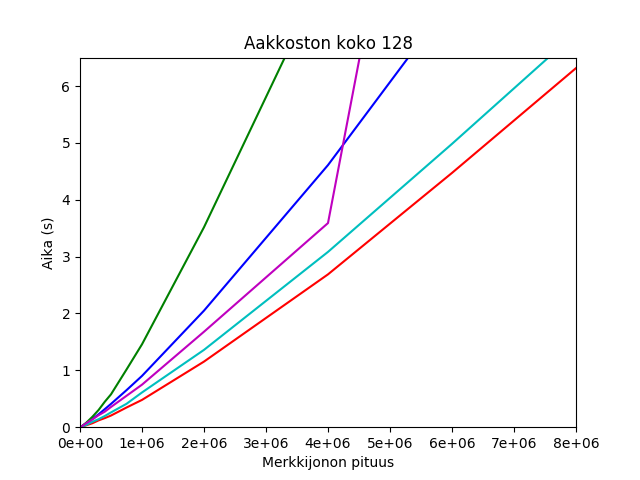
\includegraphics[width={\textwidth}]{stringlength.png}} \\ \\
            Punainen viiva: Vector  \\
            Sininen viiva: FastSet  \\
            Syaani viiva: Vector järjestystä ylläpitäen \\ 
            Violetti viiva: Taulukko  \\
            Vihreä viiva: std::set \\
            Violetti viiva (Taulukko-implementaatio) muuttaa suuntansa jyrkästi ylöspäin noin kohdassa 4000000, koska tietokoneen
            RAM-muisti loppuu sen jälkeen kesken.
            \\ \\
            Std::set ei välttämättä ole täysin vertailukelpoinen, koska edgen hakujen määrää ei ole optimoitu samalla tavalla kuin
            Vector- ja FastSet-toteutuksiossa.
            
        \newpage
        \subsection{Aakkoston koko}
        
            Kaaviossa mitatut ajat, kun syötteen koko on 2000000, aakkoston kokoa muutetaan. X-akselilla on logaritminen
            skaalaus. Aakkoston kokona on testattu tässä eri 2:n potensseja. Kuvaan on otettu joka koolta viiden kerran 
            keskiarvo. Testit on suoritettu satunnaisessa järjestyksessä, jolloin koneen suoritusnopeuden vaihtelun vaikutus
            tasoittuu.
            \\ \\
            \makebox[\textwidth]{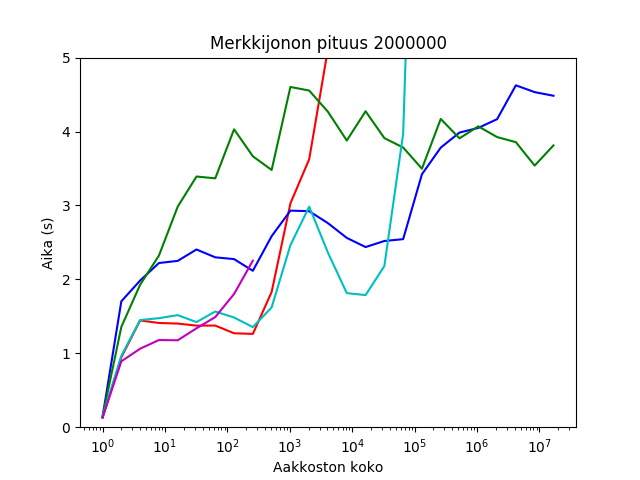
\includegraphics[width={\textwidth}]{alphabet.png}} \\ \\
            Punainen viiva: Vector  \\
            Sininen viiva: FastSet  \\
            Syaani viiva: Vector järjestystä ylläpitäen \\ 
            Violetti viiva: Taulukko  \\
            Vihreä viiva: std::set \\
            Violetti viiva (Taulukko) loppuu kesken, koska suuremmalla aakkoston koolla muistinkäyttö kasvaa liian isoksi.
            \\ \\
            Tulosten perusteella pienellä aakkostolla ($m<20$) Taulukko-ratkaisu on nopein. Aakkoston koon ollessa n. välillä
            $20<m<200$ järjestemätön vektori on nopein. Aakkoston koon kasvaessa muutamasta sadasta muutamaan tuhanteen järjestetty 
            vektor on nopein. Siitä eteenpäin FastSet ja std::set ovat selvästi nopeampia kuin muut. std::set ohittaa FastSetin
            nopeudessa vasta kohtuullisen myöhään

            Kuvassa näkyy, miten järjestettyä vectoria, FastSettiä ja std:n settiä käyttävät implementaatiot toimivat nopeammin,
            kun aakkoston koko kasvaa muutamasta tuhannesta muutamaan kymmeneen tuhanteen. Tämä johtunee siitä, että kun aakkoston
            koko on suuri suhteessa merkkijonon kokoon, puusta tulee matala ja leveä, ja edgejen pituudet (lehtiin meneviä edgejä
            tietysti lukuunottamatta) ovat lyhyitä. Tällöin tarvittavien edgejen splittausten määrä vähenee ja suurempi osa tiloista
            on jonkin noden kohdalla, jolloin siirtymien olemasasolon tutkiminen on nopeampaa.
            

    \section{Longest Common Substring}
        Longest Common Substring -algoritmin toimivuutta on yksikkötestien lisäksi testattu samankaltaisella brute-testaajalla kuin
        substring-kyselyissä. Ohjelman toiminta on tarkastettu sadoilla tuhansilla satunnaistesteillä.
\end{document}
